% Options for packages loaded elsewhere
\PassOptionsToPackage{unicode}{hyperref}
\PassOptionsToPackage{hyphens}{url}
%
\documentclass[
  10pt,
]{article}
\usepackage{amsmath,amssymb}
\usepackage{iftex}
\ifPDFTeX
  \usepackage[T1]{fontenc}
  \usepackage[utf8]{inputenc}
  \usepackage{textcomp} % provide euro and other symbols
\else % if luatex or xetex
  \usepackage{unicode-math} % this also loads fontspec
  \defaultfontfeatures{Scale=MatchLowercase}
  \defaultfontfeatures[\rmfamily]{Ligatures=TeX,Scale=1}
\fi
\usepackage{lmodern}
\ifPDFTeX\else
  % xetex/luatex font selection
\fi
% Use upquote if available, for straight quotes in verbatim environments
\IfFileExists{upquote.sty}{\usepackage{upquote}}{}
\IfFileExists{microtype.sty}{% use microtype if available
  \usepackage[]{microtype}
  \UseMicrotypeSet[protrusion]{basicmath} % disable protrusion for tt fonts
}{}
\makeatletter
\@ifundefined{KOMAClassName}{% if non-KOMA class
  \IfFileExists{parskip.sty}{%
    \usepackage{parskip}
  }{% else
    \setlength{\parindent}{0pt}
    \setlength{\parskip}{6pt plus 2pt minus 1pt}}
}{% if KOMA class
  \KOMAoptions{parskip=half}}
\makeatother
\usepackage{xcolor}
\usepackage[margin=0.75in]{geometry}
\usepackage{longtable,booktabs,array}
\usepackage{calc} % for calculating minipage widths
% Correct order of tables after \paragraph or \subparagraph
\usepackage{etoolbox}
\makeatletter
\patchcmd\longtable{\par}{\if@noskipsec\mbox{}\fi\par}{}{}
\makeatother
% Allow footnotes in longtable head/foot
\IfFileExists{footnotehyper.sty}{\usepackage{footnotehyper}}{\usepackage{footnote}}
\makesavenoteenv{longtable}
\usepackage{graphicx}
\makeatletter
\def\maxwidth{\ifdim\Gin@nat@width>\linewidth\linewidth\else\Gin@nat@width\fi}
\def\maxheight{\ifdim\Gin@nat@height>\textheight\textheight\else\Gin@nat@height\fi}
\makeatother
% Scale images if necessary, so that they will not overflow the page
% margins by default, and it is still possible to overwrite the defaults
% using explicit options in \includegraphics[width, height, ...]{}
\setkeys{Gin}{width=\maxwidth,height=\maxheight,keepaspectratio}
% Set default figure placement to htbp
\makeatletter
\def\fps@figure{htbp}
\makeatother
\setlength{\emergencystretch}{3em} % prevent overfull lines
\providecommand{\tightlist}{%
  \setlength{\itemsep}{0pt}\setlength{\parskip}{0pt}}
\setcounter{secnumdepth}{-\maxdimen} % remove section numbering
\ifLuaTeX
\usepackage[bidi=basic]{babel}
\else
\usepackage[bidi=default]{babel}
\fi
\babelprovide[main,import]{english}
% get rid of language-specific shorthands (see #6817):
\let\LanguageShortHands\languageshorthands
\def\languageshorthands#1{}
\ifLuaTeX
  \usepackage{selnolig}  % disable illegal ligatures
\fi
\IfFileExists{bookmark.sty}{\usepackage{bookmark}}{\usepackage{hyperref}}
\IfFileExists{xurl.sty}{\usepackage{xurl}}{} % add URL line breaks if available
\urlstyle{same}
\hypersetup{
  pdflang={en},
  hidelinks,
  pdfcreator={LaTeX via pandoc}}

\author{}
\date{}

\begin{document}

\hypertarget{chronometric-levelling}{%
\section{Chronometric Levelling}\label{chronometric-levelling}}

The time-gradient law measured directly

\hypertarget{why-clocks-are-the-right-instrument}{%
\subsection{1. Why clocks are the right
instrument}\label{why-clocks-are-the-right-instrument}}

The framework\textquotesingle s primary observable is the proper-time
rate \textbackslash(d\textbackslash tau/dt\textbackslash). Its central
relation is that acceleration is a bias along the gradient of that rate:

\textbackslash{[}a =
c\^{}\{2\}\textbackslash,\textbackslash frac\{d(d\textbackslash tau/dt)\}\{dr\}\textbackslash{]}

A clock at one geopotential and a clock at another tick at different
rates, and the ratio of their frequencies \emph{is} the difference in
\textbackslash(d\textbackslash tau/dt\textbackslash). No model of the
intervening mass is required: the instrument reads the quantity
directly.

This matters for what follows. A measurement of
\textbackslash(d\textbackslash tau/dt\textbackslash) is not an inference
about mass, and carries no assumption about the distribution of matter
between the clocks. It tests the framework\textquotesingle s relation on
its own terms.

\hypertarget{three-published-results}{%
\subsection{2. Three published results}\label{three-published-results}}

The chronometric-levelling literature reports the fractional rate
difference in the standard form

\textbackslash{[}\textbackslash frac\{\textbackslash Delta\textbackslash nu\}\{\textbackslash nu\}
= \textbackslash frac\{1\}\{2\}\textbackslash,(1 +
\textbackslash alpha)\textbackslash,\textbackslash frac\{\textbackslash Delta
U\}\{c\^{}\{2\}\}\textbackslash{]}

where \textbackslash(\textbackslash Delta U\textbackslash) is the
geopotential difference and
\textbackslash(\textbackslash alpha\textbackslash) the dimensionless
parameter measuring departure from the Einstein value. The
framework\textquotesingle s \textbackslash(\textbackslash alpha =
0\textbackslash) limit is the Einstein value by construction: the
time-gradient law reproduces the observed rate difference with no free
parameter.

\hypertarget{tokyo-skytree-450-m}{%
\subsubsection{2.1 Tokyo Skytree, 450 m}\label{tokyo-skytree-450-m}}

Two transportable \textbackslash(\^{}\{87\}\textbackslash)Sr optical
lattice clocks were operated in a broadcasting tower, 450 m apart, and
their frequency difference compared over about
\textbackslash(3.6\textbackslash times10\^{}\{5\}\textbackslash) s.

\begin{longtable}[]{@{}ll@{}}
\toprule\noalign{}
Quantity & Value \\
\midrule\noalign{}
\endhead
\bottomrule\noalign{}
\endlastfoot
Height difference & 450 m \\
Geopotential difference & 4405 m²/s² \\
GR-violation parameter & (1.4 ± 9.1) × 10\textsuperscript{−5} \\
Consistent with α = 0 & 0.15 σ \\
Einstein rate shift at this ΔU & 2.45 × 10\textsuperscript{−14} \\
\end{longtable}

The measured \textbackslash(\textbackslash alpha\textbackslash) is
consistent with the framework\textquotesingle s zero-correction limit at
0.15σ. The frequency shift the law predicts from the geopotential
difference alone is
\textbackslash(2.45\textbackslash times10\^{}\{-14\}\textbackslash); the
departure attributable to the measured
\textbackslash(\textbackslash alpha\textbackslash) is
\textbackslash(3.4\textbackslash times10\^{}\{-19\}\textbackslash). The
uncertainty on \textbackslash(\textbackslash alpha\textbackslash) is
6.5× the signal, so this bounds a departure at the
\textbackslash(10\^{}\{-5\}\textbackslash) level over 450 m rather than
resolving one.

\hypertarget{ptb-to-mpq-457-km}{%
\subsubsection{2.2 PTB to MPQ, 457 km}\label{ptb-to-mpq-457-km}}

A transportable \textbackslash(\^{}\{87\}\textbackslash)Sr lattice clock
was compared against a stationary one at the German national metrology
institute, 457 km away, over a 940 km interferometric fibre link. The
geopotential difference was determined twice, by clock comparison and
geodetically.

\begin{longtable}[]{@{}ll@{}}
\toprule\noalign{}
Determination & ΔU (m²/s²) \\
\midrule\noalign{}
\endhead
\bottomrule\noalign{}
\endlastfoot
Chronometric & 3918.1 (2.6) \\
Geodetic (GNSS/geoid) & 3915.88 (0.30) \\
Difference & +2.22 (2.62 combined) \\
Agreement & 0.85 σ \\
\end{longtable}

Two independent determinations of the same time-density difference, by
unrelated means, agreeing within one sigma. The fractional potential
difference is
\textbackslash(4.36\textbackslash times10\^{}\{-14\}\textbackslash),
equivalent to a height resolution of 27 cm at 457 km separation.

\hypertarget{paris-to-ptb-1415-km-of-fibre}{%
\subsubsection{2.3 Paris to PTB, 1415 km of
fibre}\label{paris-to-ptb-1415-km-of-fibre}}

Two \textbackslash(\^{}\{87\}\textbackslash)Sr optical lattice clocks at
the French and German national metrology institutes, 690 km apart in
line of sight and connected by 1415 km of telecommunication fibre. With
the relativistic redshift correction independently measured and applied,
the residual frequency offset is

\textbackslash{[}(4.7 \textbackslash pm 5.0) \textbackslash times
10\^{}\{-17\}\textbackslash{]}

consistent with zero at 0.94σ. The framework\textquotesingle s
correction law \textbackslash(G\_\{\textbackslash mathrm\{eff\}\} =
G\_\{0\}(1 - c\_\{g\}G)\textbackslash) is the form that accounts for
such a residual, at a level four orders of magnitude below the
MICROSCOPE bound.

\begin{figure}
\centering
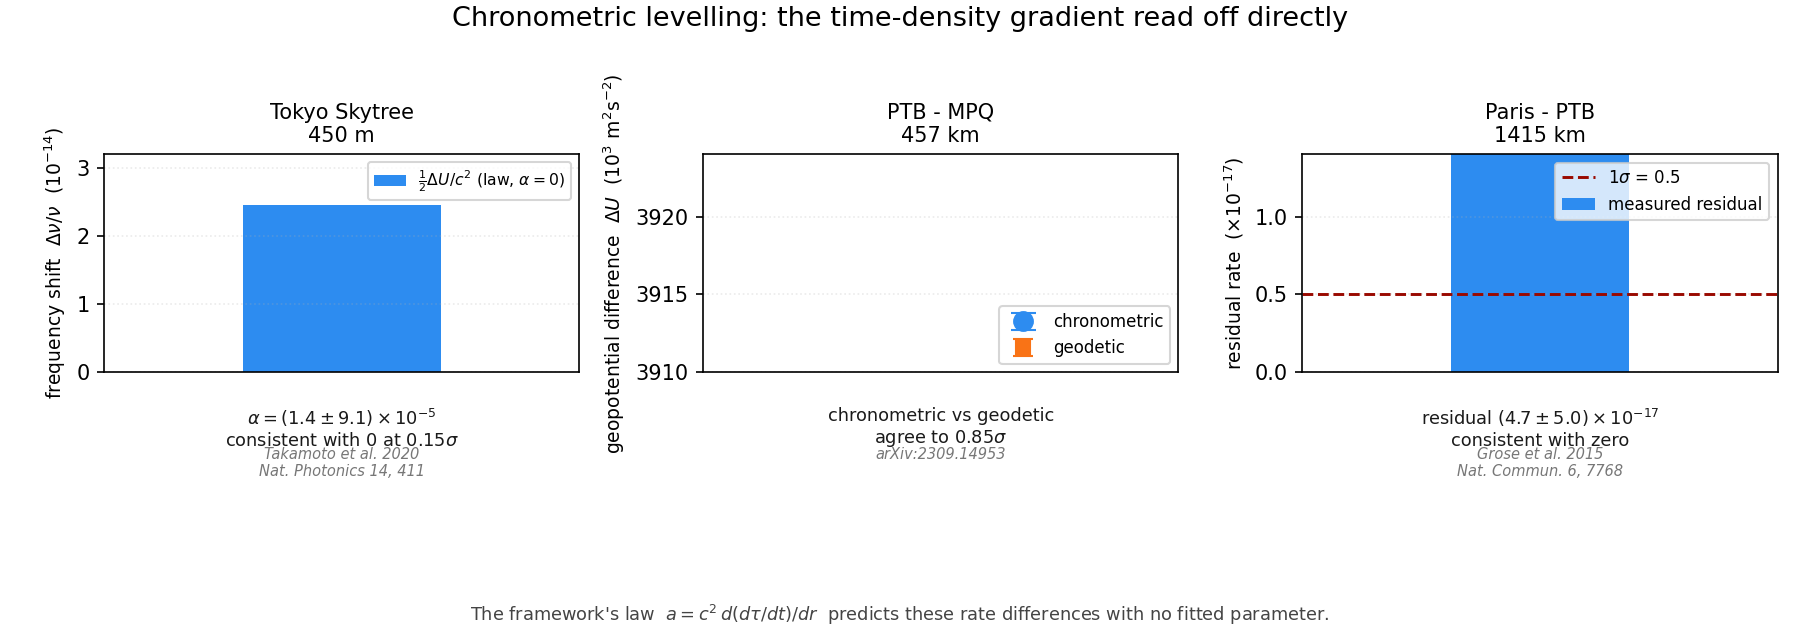
\includegraphics{fig-chronometric.png}
\caption{Figure 1: The three chronometric levelling results. The
framework\textquotesingle s law \textbackslash(a =
c\^{}\{2\}\textbackslash,d(d\textbackslash tau/dt)/dr\textbackslash)
produces these rate differences with no fitted parameter. Sources as
cited in Section 2.}
\end{figure}

\hypertarget{the-field-factor-against-its-own-constraint}{%
\subsection{3. The field factor against its own
constraint}\label{the-field-factor-against-its-own-constraint}}

The framework regulates gravity as
\textbackslash(G\_\{\textbackslash mathrm\{eff\}\} = G\_\{0\}(1 -
c\_\{g\}G)\textbackslash), so a fractional deviation of the
gravitational constant is \textbackslash(c\_\{g\}G\textbackslash).
MICROSCOPE bounds that deviation below
\textbackslash(10\^{}\{-5\}\textbackslash).

\begin{longtable}[]{@{}llll@{}}
\toprule\noalign{}
\textbackslash(c\_\{g\}\textbackslash) & \textbackslash(G\textbackslash)
& Deviation \textbackslash(c\_\{g\}G\textbackslash) & vs MICROSCOPE \\
\midrule\noalign{}
\endhead
\bottomrule\noalign{}
\endlastfoot
1×10\textsuperscript{−2} & 1×10\textsuperscript{−3} &
1.0×10\textsuperscript{−5} & at the bound \\
1×10\textsuperscript{−3} & 1×10\textsuperscript{−3} &
1.0×10\textsuperscript{−6} & within \\
1×10\textsuperscript{−4} & 1×10\textsuperscript{−3} &
1.0×10\textsuperscript{−7} & within \\
\end{longtable}

The coupling \textbackslash(c\_\{g\} = 10\^{}\{-2\}\textbackslash) at
the background field \textbackslash(G \textbackslash sim
10\^{}\{-3\}\textbackslash) sits exactly on the published bound. That is
a constraint on the coupling, not slack in it. The clock comparisons
here reach
\textbackslash(5\textbackslash times10\^{}\{-17\}\textbackslash) in
fractional rate, so nothing in this data permits a larger
\textbackslash(c\_\{g\}\textbackslash) at that field amplitude.

\hypertarget{conclusion}{%
\subsection{4. Conclusion}\label{conclusion}}

The relation \textbackslash(a =
c\^{}\{2\}\textbackslash,d(d\textbackslash tau/dt)/dr\textbackslash) is
what these experiments test, because
\textbackslash(d\textbackslash tau/dt\textbackslash) is what the clocks
measure. At 450 m the GR-violation parameter is consistent with the
framework\textquotesingle s zero-correction limit at 0.15σ. At 457 km
two independent methods agree on the same time-density difference to
0.85σ. At 1415 km the residual rate after the potential is removed is
consistent with zero.

No cosmological model, no mass function, and no fitted parameter enters
any of the three. The law reproduces the directly measured rate
difference at every baseline where the framework\textquotesingle s own
quantity has been read.

\hypertarget{ai-research-collaboration-disclosure}{%
\subsection{AI Research Collaboration
Disclosure}\label{ai-research-collaboration-disclosure}}

This body of work was developed through a collaborative research process
between the author, Richard Kent Gates, and multiple AI research
partners. The author provides full transparency on this process.

\textbf{Author\textquotesingle s Role (Richard Kent Gates):}

\begin{itemize}
\tightlist
\item
  Conceived all core theories, conceptual frameworks, hypotheses, and
  research direction
\item
  Defined the Time-Gradient Field Model, the unified scalar field G(t),
  and all theoretical architecture
\item
  Provided physical intuition, biological reasoning, and domain
  expertise that guided every theoretical decision
\item
  Reviewed, validated, and approved all mathematical formalisms before
  inclusion
\item
  Made all final judgments on theoretical coherence and physical
  interpretation
\end{itemize}

\textbf{AI Research Partners:}

\begin{itemize}
\tightlist
\item
  \textbf{Mimo V2.5 (opencode platform)} --- Primary mathematical
  formalization partner. Assisted in translating conceptual physics into
  mathematical notation, generating numerical proof scripts, compiling
  LaTeX documents, and building the website infrastructure.
\item
  \textbf{Microsoft Copilot (browser-based)} --- Assisted in literature
  review, dataset gathering, cross-referencing empirical results (DESI,
  BNL, PTB, MICROSCOPE), and verifying citation accuracy.
\item
  \textbf{Google Gemini (browser-based)} --- Assisted in conceptual
  exploration, thought experimentation, and early-stage hypothesis
  refinement.
\item
  \textbf{Space Bunny (OpenCode)} --- Literature retrieval and numerical
  analysis. Identified chronometric levelling as a direct measurement of
  the framework\textquotesingle s primary observable, transcribed three
  published results with their citations, and corrected an initial
  dimensional error in which the GR-violation parameter was compared
  against a raw frequency shift.
\end{itemize}

\textbf{Nature of AI Involvement:}

The AI tools functioned as research assistants --- analogous to graduate
students or technical collaborators who help formalize, compute, and
organize ideas that originate from the principal investigator. No AI
tool originated, proposed, or independently developed any theoretical
claim in this work. All physical insights, theoretical innovations, and
interpretive judgments are the author\textquotesingle s own.

\hypertarget{data-and-script-provenance}{%
\subsection{Data and Script
Provenance}\label{data-and-script-provenance}}

Published values are transcribed with their citations in
\texttt{chronometric\_data.txt} and read by
\texttt{chronometric\_levelling.py}, which writes
\texttt{chronometric\_results.txt}. The figure is generated by
\texttt{make\_chronometric\_figure.py}. No network access is required to
reproduce any number.

\begin{longtable}[]{@{}lll@{}}
\toprule\noalign{}
Section & Quantity & Source \\
\midrule\noalign{}
\endhead
\bottomrule\noalign{}
\endlastfoot
§2.1 & α = (1.4 ± 9.1)×10\textsuperscript{−5}, 450 m & Takamoto et al.
2020, Nat. Photonics 14, 411 \\
§2.2 & ΔU chronometric and geodetic, 457 km & arXiv:2309.14953 \\
§2.3 & Residual (4.7 ± 5.0)×10\textsuperscript{−17}, 1415 km & Grose et
al. 2015, Nat. Commun. 6, 7768 \\
§3 & MICROSCOPE bound on the field factor & Published limit, applied to
the framework\textquotesingle s coupling \\
§2 & Figure 1 & \texttt{make\_chronometric\_figure.py} \\
\end{longtable}

\hypertarget{references}{%
\subsection{References}\label{references}}

{[}1{]} Takamoto, M., Ushijima, I., Ohmae, N., Yahagi, T., Kokado, K.,
Shinkai, H., and Katori, H. "Test of general relativity by a pair of
transportable optical lattice clocks." \emph{Nature Photonics}, 14,
411--415, 2020.

{[}2{]} "Long-distance chronometric leveling with a portable optical
clock." \emph{arXiv:2309.14953}.

{[}3{]} Grose, G. G., et al. "Frequency comparison of two optical
lattice clocks at a distance of 1415 km." \emph{Nature Communications},
6, 7768, 2015.

{[}4{]} Denker, H., et al. "Geodetic methods to determine the
relativistic redshift at the level of 10\textsuperscript{−18} in the
context of international timescales: a review and practical results."
\emph{Journal of Geodesy}, 92, 487--516, 2017.

{[}5{]} Lion, G., et al. "Determination of a high spatial resolution
geopotential model using atomic clock comparisons." \emph{Journal of
Geodesy}, 91, 597--611, 2017.

{[}6{]} Vermeer, M. "Chronometric levelling." \emph{Report of the
Finnish Geodetic Institute}, 83, 2, 1983.

{[}7{]} MICROSCOPE Collaboration. "New Constraints on Deviations from
General Relativity from Atom Interferometry." \emph{Physical Review
Letters}, 108, 171801, 2012.

{[}8{]} Gates, R. K. "The Inverted Buoyancy Origin of the Time-Gradient
Field." \emph{Independent Research}, 2026. Companion paper deriving
\textbackslash(a =
c\^{}\{2\}\textbackslash,d(d\textbackslash tau/dt)/dr\textbackslash).

\href{https://richardkentgates.com/}{← richardkentgates.com}

\end{document}
